\section{Diskusjon}

\subsection{Måling på RC-ledd}
\subsubsection{Én kondensator}
Signalgeneratoren ble stilt inn på $f=150\text{Hz}$ og amplituden målte $1.0\text{V{p-p}}$ på oscilloskopet. Kretsen under viser målingsutgangspunktet.

\begin{figure}[H]
\centering
\begin{circuitikz}[american voltages]

    \node[circle, fill=black, inner sep=1.2pt] (A)  at (0,0) {};
    \node[circle, fill=black, inner sep=1.2pt] (B)  at (0,4) {};
    \node[circle, fill=black, inner sep=1.2pt] (C)  at (8,4) {};
    \node[circle, fill=black, inner sep=1.2pt] (D)  at (8,0) {};

    \node at (A) [ground] {};
    \node at (D) [ground] {};
    \node[above left] at (B) {$A$};
    \node[above right] at (C) {$B$};
    \node[above right] at (D) {$C$};

    \draw (A) to[sV, l_=$V_1$] (B);
    \draw (B) to[R, l_=$R_4$, a^=$1\text{k}\Omega$] (C);
    \draw (C) to[C, l_=$C_7$, a^=$470\text{nF}$] (D);

\end{circuitikz}
\caption{RC krets med én kondensator.}
\end{figure}

\noindent
Resultatet i figur~\ref{fig:rc_ledd_alene} gir et godt bilde av hva som er spenningen over kondensatoren i forhold til spenningskilden. Spenningen i kondensatoren vil nærme seg firkantpulsen eksponensielt og resultatet kan vi si er godt innafor. Videre kan vi se på spenningen over motstanden $R_4$. For å kunne måle spenningen over denne motstanden må vi gjøre om på kretsen for å unngå å måle over ingen spenningsforskjell. Kretsen blir nå seende slik ut.
\begin{figure}[H]
\centering
\begin{circuitikz}[american voltages]

    \node[circle, fill=black, inner sep=1.2pt] (A)  at (0,0) {};
    \node[circle, fill=black, inner sep=1.2pt] (B)  at (0,4) {};
    \node[circle, fill=black, inner sep=1.2pt] (C)  at (8,4) {};
    \node[circle, fill=black, inner sep=1.2pt] (D)  at (8,0) {};

    \node at (A) [ground] {};
    \node at (D) [ground] {};
    \node[above left] at (B) {$A$};
    \node[above right] at (C) {$B$};
    \node[above right] at (D) {$C$};

    \draw (A) to[sV, l_=$V_1$] (B);
    \draw (C) to[R, l_=$R_4$, a^=$1\text{k}\Omega$] (D);
    \draw (B) to[C, l_=$C_7$, a^=$470\text{nF}$] (C);

\end{circuitikz}
\caption{Krets for måling av RC-ledd.}
\end{figure}

\noindent
Resultatet i figur~\ref{fig:spenning_R4} kan vi også si er riktig. Dette er fordi grafen kan forklares med å se på strømmen gjennom motstanden. Siden spenningen over motstanden beskrives som $V_R(t)$ = $R_4i(t)$. I et RC-ledd vil strømmen bestemmes av derivert spenning over kondensatoren:
\[
\begin{aligned}
    i(t)&=C\frac{dv_C(t)}{dt} \\
    v_R(t)&=RC\frac{dv_C(t)}{dt}
\end{aligned}
\]
\noindent
Nå kan vi se at spenningen over motstanden bestemmes av endringen i spenningen i kondensatoren. Derfor vil det bli stor spenning over motstanden når kondensatorspenningen stiger eller faller raskt. Når spenningen over kondensatoren flater ut vil derfor $V_R(t)$ eksponentielt synke mot null. Vi kan grafe $V_C(t)$, $V_1(t)$ og $V_R(t)$ for å se forholdet mellom dem. Ved å bruke de kjente verdiene og sette dem inn i ligning~\ref{eq:spenning_i_kondensator}.

\[
\tau = R_4 \cdot C_7 = 0.470\text{ms}
\]
\[
V_F = 1.0\text{V}
\]

\[
\begin{aligned}
v_C(t) &=
\begin{cases}
1 -  e^{-{t}/{0.470\text{ms}}}, 
    & 0 \le t \le 10\text{ms},\\[0.5em]
e^{-\left(t - 10\text{ms}\right)/{0.470\text{ms}}}, 
    & 10\text{ms} \le t \le 20\text{ms},
\end{cases}
\end{aligned}
\]

\[
v_R(t) = R_4C_7\cdot v_C'(t)
\]

\[
\begin{aligned}
v_R(t) &=
\begin{cases}
e^{-{t}/{0.470\text{ms}}}, 
    & 0 \le t \le 10\text{ms},\\[0.5em]
-e^{-\left(t - 10\text{ms}\right)/{0.470\text{ms}}}, 
    & 10\text{ms} \le t \le 20\text{ms},
\end{cases}
\end{aligned}
\]


\begin{figure}[H]
\centering
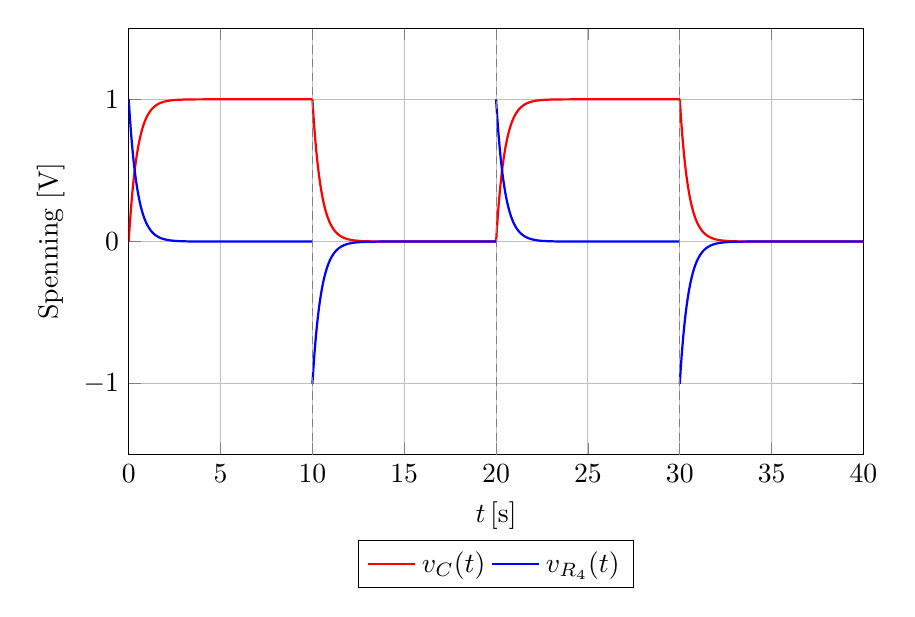
\begin{tikzpicture}
\begin{axis}[
    width=0.9\textwidth,
    height=7cm,
    xlabel={$t\,[\mathrm{s}]$},
    ylabel={Spenning\ [V]},
    xmin=0, xmax=40,
    ymin=-1.5, ymax=1.5,
    grid=both,
    legend style={at={(0.5,-0.2)},anchor=north,legend columns=2},
    samples=200
]

    % --- v_C(t): spenning over kondensatoren ---
    % Periode 1: 0–20 s
    \addplot[
        thick,
        red,
        domain=0:10
    ]
        {(1 - exp(-x/0.470))};
    \addplot[
        thick,
        red,
        domain=10:20,
        forget plot
    ]
        {exp(-(x-10)/0.470)};
    % Periode 2: 20–40 s
    \addplot[
        thick,
        red,
        domain=20:30,
        forget plot
    ]
        {(1 - exp(-(x - 20)/0.470))};
    \addplot[
        thick,
        red,
        domain=30:40,
        forget plot
    ]
        {exp(-(x-30)/0.470)};
    \addlegendentry{$v_C(t)$}

    % --- v_R4(t): spenning over motstanden R4 ---
    % Periode 1: 0–20 s
    \addplot[
        thick,
        blue,
        domain=0:10
    ]
        {exp(-x/0.470)};
    \addplot[
        thick,
        blue,
        domain=10:20,
        forget plot
    ]
        {-exp(-(x-10)/0.470)};
    % Periode 2: 20–40 s
    \addplot[
        thick,
        blue,
        domain=20:30,
        forget plot
    ]
        {exp(-(x-20)/0.470)};
    \addplot[
        thick,
        blue,
        domain=30:40,
        forget plot
    ]
        {-exp(-(x-30)/0.470)};
    \addlegendentry{$v_{R_4}(t)$}

    % Vertikale hjelpelinjer (valgfritt, ikke i legend)
    \addplot[
        gray,
        densely dashed,
        forget plot
    ]
        coordinates {(10,-1.5) (10,1.5)};
    \addplot[
        gray,
        densely dashed,
        forget plot
    ]
        coordinates {(20,-1.5) (20,1.5)};
    \addplot[
        gray,
        densely dashed,
        forget plot
    ]
        coordinates {(30,-1.5) (30,1.5)};

\end{axis}
\end{tikzpicture}
\caption{Teoretisk spenning over kondensatoren $C_T$ og motstanden $R_4$ for et firkantet inngangssignal med periode $20\,\text{s}$ og tidskonstant $\tau = 0{,}47\,\text{s}$.}
\end{figure}

\noindent
Siden dette er teoretisk tilnærming med verdiene vi har er ikke grafen helt lik den på oscilloskopet. Uansett, så bekrefter den at grafene henger sammen. Utledningen av at spenningen over motstanden er proporsjonal med endringen i spenningen på kondensatoren stemmer overens med grafen.









\subsubsection{To kondensatorer i serekobling}

\begin{figure}[H]
\centering
\begin{circuitikz}[american voltages]

    \node[circle, fill=black, inner sep=1.2pt] (A)  at (0,0) {};
    \node[circle, fill=black, inner sep=1.2pt] (B)  at (0,4) {};
    \node[circle, fill=black, inner sep=1.2pt] (C)  at (8,4) {};
    \node[circle, fill=black, inner sep=1.2pt] (D)  at (8,0) {};

    \node at (A) [ground] {};
    \node at (D) [ground] {};
    \node[above left] at (B) {$A$};
    \node[above right] at (C) {$B$};
    \node[above right] at (D) {$C$};

    \draw (A) to[sV, l_=$V_1$] (B);
    \draw (B) to[R, l_=$R_4$, a^=$1\text{k}\Omega$] (C);

    \draw (C) to[C, l_=$C_7$, a^=$470\text{nF}$] (8,2);
    \draw (8,2) to[C, l_=$C_8$, a^=$470\text{nF}$] (D);

\end{circuitikz}
\caption{RC krets med to kondensatorer i seriekobling}
\end{figure}

Resultatet på oscilloskopet i figur~\ref{fig:rc_ledd_ser} er et godt bilde av teorien. Vi må se på  totalkapasitanten for å besvare hvorfor. Totalkapasitansen i serie regnes på formen: $C_{tot}^{-1} = C_1^{-1} + \dots + C_N^{-1}$. I denne kretsen vil da totalkapasitansen være.
\[
\begin{aligned}
    C_{tot}^{-1} &= C_7^{-1} + C_8^{-1} \\
    C_{tot}^{-1} &= 2\cdot\left(470\text{nF}\right)^{-1} \\
    C_{tot} &= 235\text{nF}
\end{aligned}
\]
\noindent
Dette betyr at siden totalkapasitansen er lavere vil da tidskonstanten også være lavere, kondensatoren vil ha en lavere oppladings- og nedladingstid. Resultatet viser akkurat dette sammenliknet med bare én kondensator, siden tidskonstanten er lavere vil endringen i spenning være raskere.








\subsubsection{To kondensatorer i parallellkobling}

\begin{figure}[H]
\centering
\begin{circuitikz}[american voltages]

    \node[circle, fill=black, inner sep=1.2pt] (A)  at (0,0) {};
    \node[circle, fill=black, inner sep=1.2pt] (B)  at (0,4) {};
    \node[circle, fill=black, inner sep=1.2pt] (C)  at (8,4) {};
    \node[circle, fill=black, inner sep=1.2pt] (D)  at (4,0) {};
    \node[circle, fill=black, inner sep=1.2pt] (BL)  at (4,4) {};
    \node[circle, fill=black, inner sep=1.2pt] (DR)  at (8,0) {};

    \node at (A) [ground] {};
    \node at (D) [ground] {};
    \node[above left] at (B) {$A$};
    \node[above right] at (C) {$B$};
    \node[above right] at (D) {$C$};

    \draw (BL) -- (C);
    \draw (DR) -- (D);

    \draw (A) to[sV, l_=$V_1$] (B);
    \draw (B) to[R, l_=$R_4$, a^=$1\text{k}\Omega$] (BL);
    \draw (BL) to[C, l_=$C_7$, a^=$470\text{nF}$] (D);
    \draw (C) to[C, l_=$C_8$, a^=$470\text{nF}$] (DR);

\end{circuitikz}
\caption{RC krets med to kondensatorer i parallellkobling. }
\end{figure}

For å besvare hvorfor dette resultatet er et riktig bilde av teorien må vi se på totalkapasitanten. Totalkapasitansen her representeres av $C_1$ og $C_2$ i parallellkobling. Kondensatorer i parallellkobling vil gi en totalkapasitans av summen av dem.
\[
\begin{aligned}
    C_{tot} &= 470\text{nF} + 470\text{nF} \\
    C_{tot} &= 940\text{nF}
\end{aligned}
\]

\noindent
Denne totalkapasitanten forteller oss at tidskonstanten vil være høyere enn hva den vil være hvis det var én kondensator alene. Derfor vil kondensatorene her lades og utlades på en lavere hastighet enn ved seriekoblede kondensatorer. Derfor vil dette resultatet være et bra bilde.






\subsubsection{Sammenlikning av tilfellene}










\subsection{Måling av RL-ledd}
Kretsen for målingen av spole induktans er som i kretsen i figur~\ref{fig:rl-ledd}. Innstillingene for funksjonsgeneratoren er frekvens, $f = 100 \text{kHz}$ og amplitude slik at oscilloskopet måler $1.0V_{\text{pp}}$.
\begin{figure}[H]\label{fig:rl-ledd}
\centering
\begin{circuitikz}[american voltages]

    \node[circle, fill=black, inner sep=1.2pt] (A)  at (0,0) {};
    \node[circle, fill=black, inner sep=1.2pt] (B)  at (0,4) {};
    \node[circle, fill=black, inner sep=1.2pt] (C)  at (8,4) {};
    \node[circle, fill=black, inner sep=1.2pt] (D)  at (8,0) {};

    \node at (A) [ground] {};
    \node at (D) [ground] {};

    \node [above left] at (B) {$A$};
    \node [above right] at (C) {$B$};
    \node [right] at (D) {$C$};

    \draw (A) to[sV, l_=$V_2$, a^=$1.0 V_{pp}$] (B);

    \draw (B) to[L, l_=$L_2$, a^=$47\text{\textmu}\text{H}$] (C);

    \draw (C) to[R, l_=$R_2$, a^=$51\Omega$] (D);
    

\end{circuitikz}
\caption{Krets for måling av RL-ledd.}
\end{figure}

\noindent
Resultatene er uklare og viser ikke det ekte forholdet mellom grafene. Denne kretsen presenterer en RL-krets som består av en AC-spenningskilde, spole og motstand. I en krets som dette vil spolen motvirke endring i strøm ved å indusere en spenning. Denne spenningen vil bli synlig på oscilloskopet i totalspenningen. Ser vi på resultatene kan vi først ta for oss målingen av spenning over motstand og totalspenningen.
\\[1em]
\noindent
Resultatet er ikke riktig i form av avbilding, grafene er ikke riktig innstilt i forhold til amplitudene. Ideelt sett, dersom spenningskilden hadde vært perfekt, skulle totalspenningen i kretsen vært en ren firkantpuls, mens spenningen over motstanden skulle fulgt en eksponentiell opp- og nedgang bestemt av tidskonstanten $\tau = L / (R + R_s)$. Målingene viser derimot at totalspenningen får en tydelig topp rett etter hver overgang, og at kurven glatter seg inn mot et nivå som er lavere enn toppverdien. Samtidig ser vi at spenningen over motstanden følger den forventede eksponentielle formen, men at den ligger noe lavere enn totalspenningen i starten av pulsen.
\\[1em]
\noindent
Dette kan forklares ved at funksjonsgeneratoren i praksis ikke er en ideell spenningskilde, men har en intern motstand på omtrent $50\Omega$ og begrenset stige- og falltid. Når firkantpulsen går fra lav til høy, forsøker strømmen i kretsen å øke momentant. Spolen motvirker denne endringen ved å indusere en spenning:

\[
v_L = L\cdot \frac{di}{dt}
\]
\noindent
Denne induserte spenningen legger seg oppå kildespenningen og gjør at den målte totalspenningen får en kortvarig topp (oversving) før den avtar eksponentielt mot et stasjonært nivå. Når pulsen går fra høy til lav skjer det motsatte: spolen forsøker å opprettholde strømmen og induserer en spenning med motsatt fortegn, noe som gir et negativt “dropp” i totalspenningen.
\\[1em]
\noindent
Summen av spenningen over motstanden og spenningen over spolen er likevel lik kildespenningen til enhver tid. Det betyr at målingene er konsistente med teorien dersom vi tar hensyn til kildeimpedansen og at spenningskilden ikke er ideell. Dette forklarer hvorfor oscilloskopbildet ikke viser en perfekt firkantpuls som totalspenning, men en puls med tydelige topper ved overgangene, samtidig som formen på spenningen over motstanden stemmer godt med den teoretiske RL-responsen.
\\[1em]
\noindent
I figuren under viser vi den teoretiske spenningen over motstanden, spolen og totalspenningen i kretsen. 
Den teoretiske responsen er basert på standardligningen for en seriekoblet RL-krets
\[
L\frac{di}{dt} + (R + R_s)\,i(t) = V_s(t),
\]
der $R_s$ er funksjonsgeneratorens interne motstand. Løsningen gir en eksponentiell strømrespons med 
tidskonstant 
\[
\tau = \frac{L}{R + R_s}.
\]
Spenningene som plottes er deretter beregnet som 
\[
v_R(t) = i(t)R, \qquad 
v_L(t) = L\,\frac{di}{dt}, \qquad 
v_{\text{tot}}(t) = V_s(t) - i(t)R_s.
\]
Disse teoretiske kurvene stemmer godt overens med måleresultatene, spesielt når vi tar hensyn til 
kildeimpedansen og oscilloskopets skaleringsfeil.


\begin{figure}[H]
\centering
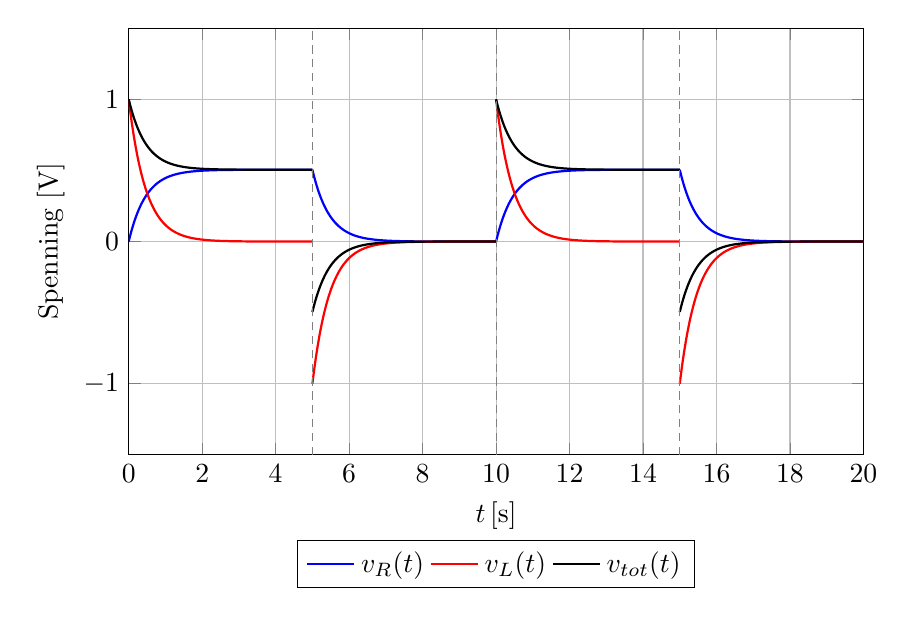
\begin{tikzpicture}
\begin{axis}[
    width=0.9\textwidth,
    height=7cm,
    xlabel={$t\,[\mathrm{\text{\textmu}s}]$},
    ylabel={Spenning\ [V]},
    xmin=0, xmax=20,
    ymin=-1.5, ymax=1.5,
    grid=both,
    legend style={at={(0.5,-0.2)},anchor=north,legend columns=3},
    samples=200
]

    % Parametre (i mikrosekund): T = 10 µs, T/2 = 5 µs, tau ≈ 0.465 µs
    % Rs = 50 Ω, R = 51 Ω
    % DC-nivåer: R/(R+Rs) ≈ 0.50495, Rs/(R+Rs) ≈ 0.49505

    % v_R(t): spenning over motstanden
    % Periode 1: 0–10 µs
    \addplot[
        thick,
        blue,
        domain=0:5
    ]
        {0.50495*(1 - exp(-x/0.465))};          % 0 <= t < 5 us
    \addplot[
        thick,
        blue,
        domain=5:10,
        forget plot
    ]
        {0.50495*exp(-(x-5)/0.465)};            % 5 <= t < 10 us
    % Periode 2: 10–20 µs
    \addplot[
        thick,
        blue,
        domain=10:15,
        forget plot
    ]
        {0.50495*(1 - exp(-(x-10)/0.465))};     % 10 <= t < 15 us
    \addplot[
        thick,
        blue,
        domain=15:20,
        forget plot
    ]
        {0.50495*exp(-(x-15)/0.465)};           % 15 <= t < 20 us
    \addlegendentry{$v_R(t)$}

    % v_L(t): spenning over spolen
    % Periode 1: 0–10 µs
    \addplot[
        thick,
        red,
        domain=0:5
    ]
        {exp(-x/0.465)};                        % 0 <= t < 5 us
    \addplot[
        thick,
        red,
        domain=5:10,
        forget plot
    ]
        {-exp(-(x-5)/0.465)};                   % 5 <= t < 10 us
    % Periode 2: 10–20 µs
    \addplot[
        thick,
        red,
        domain=10:15,
        forget plot
    ]
        {exp(-(x-10)/0.465)};                   % 10 <= t < 15 us
    \addplot[
        thick,
        red,
        domain=15:20,
        forget plot
    ]
        {-exp(-(x-15)/0.465)};                  % 15 <= t < 20 us
    \addlegendentry{$v_L(t)$}

    % v_tot(t): spenning over hele RL-leddet (det som måles som "totalspenning")
    % Periode 1: 0–10 µs
    \addplot[
        thick,
        black,
        domain=0:5
    ]
        {0.50495 + 0.49505*exp(-x/0.465)};      % 0 <= t < 5 us
    \addplot[
        thick,
        black,
        domain=5:10,
        forget plot
    ]
        {-0.49505*exp(-(x-5)/0.465)};           % 5 <= t < 10 us
    % Periode 2: 10–20 µs
    \addplot[
        thick,
        black,
        domain=10:15,
        forget plot
    ]
        {0.50495 + 0.49505*exp(-(x-10)/0.465)}; % 10 <= t < 15 us
    \addplot[
        thick,
        black,
        domain=15:20,
        forget plot
    ]
        {-0.49505*exp(-(x-15)/0.465)};          % 15 <= t < 20 us
    \addlegendentry{$v_{\text{tot}}(t)$}

    % Vertikale hjelpelinjer for T/2 og T
    \addplot[
        gray,
        densely dashed,
        forget plot
    ]
        coordinates {(5,-1.5) (5,1.5)};
    \addplot[
        gray,
        densely dashed,
        forget plot
    ]
        coordinates {(10,-1.5) (10,1.5)};
    \addplot[
        gray,
        densely dashed,
        forget plot
    ]
        coordinates {(15,-1.5) (15,1.5)};

\end{axis}
\end{tikzpicture}
\caption{Teoretisk spenning over spolen $L$, motstanden $R$ og totalspenningen $v_{\text{tot}}(t)$ i RL-kretsen med intern kilde\-motstand $R_s = 50\,\Omega$. Inngangssignalet er en firkantpuls med periode $T = 10\,\mathrm{\text{\textmu}s}$ og tidskonstant $\tau \approx 0{,}465\,\mathrm{\text{\textmu}s}$.}
\end{figure}




\subsection{Krets med RC-ledd}
Dette resultatet kommer fra teorien i~\ref{subsec:rc-krets-teori}. Resultatene presenterer målinger av akkurat denne kretsen med samme firkantpuls på spenningskilden. Resultatene må sammenliknes med figur~\ref{fig:teor_vC_ogv0}, og vi ser at resultatene stemmer. Grafen vokser og synker presist som teorien foreslår, og amplituden er riktig på både $v_c(t)$ og $v_0(t)$. Avviket er $0.16\%$ på målingen for $v_c(t)$ med en teoretisk verdi på $6.07$ og en praktisk måling på $6.08$. Avviket for $v_0(t)$ er $1.44\%$ med en praktisk måling på 2.82V og en teoretisk verdi på 2.78V. Resultatene kan vi derfor påstå at er gode og pålitelige. Grafene er riktig.
\\[1em]
Sammenhengen mellom grafene er også viktig å analysere. For å svare på hvorfor selve funksjonsoppførselen er lik, men amplituden er annerledes må vi ser på kretsen i figur~\ref{fig:krets-med-rc-ledd}. Spenningen for kondensatoren er gitt ved spenningen i node A, og spenningen over $3.3\text{k}\Omega$ motstanden er begge gitt ved to forskjellige spenningsdelere. Node A vil matematisk ha høyere spenning enn $v_0$. Dermed vil grafene oppføre seg likt i form av øking og synking, men med forskjellig hastighet og vil dermed få forskjellig amplitude i spenningen.